\section{Failure Analysis}
\label{sec:failures}

We took every run of the full system that ended without a correct program and assigned it to one category, using the last oracle verdict, the last verifier diagnostics and the final program. The categories and their frequencies are shown in Fig.~\ref{fig:failures}.

\begin{figure}[t]
\centering
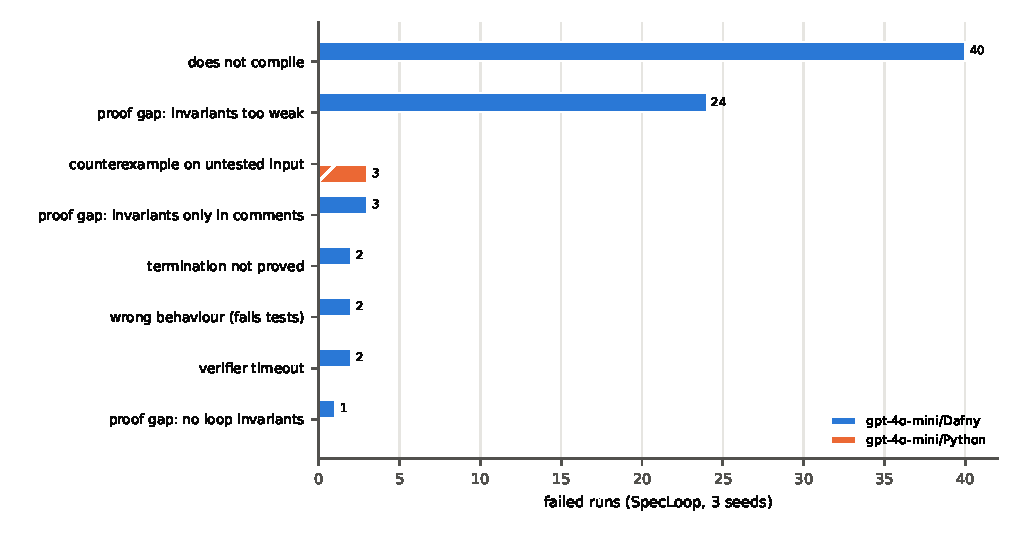
\includegraphics[width=\columnwidth]{generated/fig_failures.pdf}
\caption{Failure categories of the full SpecLoop agent on the test split (all failed runs over three seeds).}
\label{fig:failures}
\end{figure}

Over three seeds the full agent failed \R{fail.dafny.total} Dafny runs and \R{fail.python.total} Python runs. Four categories cover almost all of them.

\textbf{Does not compile (\R{fail.dafny.DoesNotCompile} Dafny runs, \R{fail.dafny.DoesNotCompile.share}\%).} The most frequent failure is a program that never compiles, even after four repairs. The errors are the ones that motivated development iteration~4: array operations on sequences, string building with constructs Dafny does not have, statement \texttt{if} written with \texttt{then}, and calls to library functions that do not exist. The fix hints help (vb\_017, vb\_082 and vb\_105 were solved on the dev split only after they were added), but GPT-4o-mini often swaps one compile error for another instead of converging. This mirrors VERINA, where most GPT-4o-mini failures were Lean compile errors. Better language grounding, for example retrieving short Dafny idioms for the construct that failed, is the obvious next step.

\textbf{Proof gap (\R{fail.dafny.ProofGapInvariantsTooWeak} + \R{fail.dafny.ProofGapInvariantsOnlyInComments} + \R{fail.dafny.ProofGapNoLoopInvariants} runs).} The program passes every test but does not verify. In most of these runs the invariants exist but are too weak to imply the postcondition, typically a bound on the index without a clause that relates the partial result to the specification. A few runs still write the invariants as comments or leave them out entirely. Here the router does its job and labels these attempts \textsc{proof\_gap}, but the model does not know how to strengthen the invariant. Invariant-generation techniques such as those in Lemur~\cite{wu2024lemur} or Laurel~\cite{mugnier2025laurel} would slot into exactly this branch of the loop.

\textbf{Termination and timeouts (\R{fail.dafny.TerminationNotProved} + \R{fail.dafny.VerifierTimeout} runs).} Missing \texttt{decreases} clauses and quantifier-heavy invariants that exhaust the verifier's time limit are rare with these small tasks.

\textbf{Wrong behaviour and counterexamples (\R{fail.dafny.WrongBehaviourFailsTests} Dafny, \R{fail.python.CounterexampleOnUntestedInput} Python runs).} Very few runs end with code that is actually wrong. In Python every failure is a program that passes all tests but for which CrossHair finds an input that breaks a contract, which is precisely the kind of error the verifier is there to catch.

\textbf{Representative cases.} The trajectories are in \texttt{results/cases/} of the repository. \emph{Success 1} (vb\_016, Dafny, replace characters): the first candidate does not compile (array syntax on a sequence) and is routed as \textsc{syntax}. The second compiles and passes every visible test but does not verify, so the router labels it \textsc{proof\_gap}. The model keeps the algorithm, adds an invariant that ties the partial result to the input, and the third candidate verifies. \emph{Success 2} (vb\_033, Python, smallest missing number): the first candidate passes all five tests, but CrossHair finds a sorted input with duplicates that breaks the postcondition (\textsc{logic\_bug}). The next candidate fails in the same way, the stagnation monitor switches to a rewrite, and the rewritten set-based version is correct. A testing-only agent would have stopped at the first, wrong program. \emph{Failure 1} (vb\_009, Dafny, common element): the code is right from the first attempt and passes all eight tests, but all five candidates fail on invariants about the multiset of seen elements; each repair changes the invariants without making them strong enough. \emph{Failure 2} (vb\_086, Dafny, rotate a sequence): the first candidate tries to fill an array where the specification works with sequences, the second and third use a comprehension syntax that does not exist in Dafny, and the fourth goes back to a resolution error. All four are routed as \textsc{syntax}. The fifth candidate finally compiles but rotates in the wrong direction and passes only one of six tests.
